\chapter{Results}
\label{ch:results}
%
% The scope of this thesis includes the generation, animation and rendering of the
% surface of an open ocean in real-time. We focus our interest on the synthesis of
% animated ocean surface geometry, for which we will adopt a set of models from
% oceanographic research.

The previous chapter discussed in detail the approach we took to synthesize
the animated ocean surface, including, one, a number of optimizations to reduce
the computational workload, and, two, a level of detail mechanism which does
not only give us fine-grained control over model detail, but also allows us to
reduce potential tiling artifacts. Additionally, we gave an overview of our demo
application, which integrates our approach to ocean surface synthesis
with real-time rendering algorithms which have been developed specifically for
the display of the open ocean.
Thus, with our demo application at hand, we may move on to discuss the
actual results we were able to achieve.

The remainder of this chapter is organized as follows:
Section \ref{sec:results:performance} gives a compact overview of the performance
improvements which we were able to attain for the generation of the ocean
surface spectra as well as for the computation of the sum of waves via the
\InvFourierTransform.
Section \ref{sec:results:synthesis} delineates the pitfalls we encountered
in the context of ocean surface synthesis with wave spectra, and what measures
we took to either overcome or sidestep them.
Last, Section \ref{sec:results:fidelity} discusses the level of visual fidelity
we were able to obtain, with focus on the different wave spectra, as well as
our level of detail approach.
% Before we delve into details, one may look at Figure~\ref{fig:results} which
% depicts all componenents which are part of our ocean lighting implementation.
% compare lighting of all spectrum types (same parameters)
%
\section{Performance}
\label{sec:results:performance}
%
% \begin{table}
% \centering
% \begin{tabular}{@{}l*2{S[table-format=1.2]}*2{S[table-format=2.2]}*2{S[table-format=3.2]}@{}}
% \toprule
% Spectrum & \multicolumn{6}{c}{Time [\si{\ms}]}       \\ \midrule
%          & \multicolumn{6}{c}{Resolution} \\ \cmidrule(l){2-7} 
%          & {$32\times32$} & {$64\times64$}  & {$128\times128$}  & {$256\times256$}  & {$512\times512$} & {$1024\times1024$} \\
% \midrule
% \csvreader[late after line=\\,late after last line=\\\bottomrule]{figures/benchmark_H0_i5_5300u.csv}{}{\csvcoli & \csvcoliv & \csvcolv & \csvcolvi & \csvcolvii & \csvcolviii & \csvcolix}
% \end{tabular}
% \caption{Computation times for the static part of the spectrum at various resolutions
% with different underlying wave energy spectra. One can see that at larger resolutions
% we would be unable to synthesize the static part of the spectrum more than a few times
% a second, much less so in case of more than one level of detail.}
% \label{tab:results:h0}
% \end{table}
%
% \begin{table}
% \centering
% \begin{tabular}{@{}l*2{S[table-format=1.2]}*2{S[table-format=2.2]}*2{S[table-format=3.2]}@{}}
% \toprule
% Spectrum & \multicolumn{6}{c}{Time [\si{\ms}]}       \\ \midrule
%          & \multicolumn{6}{c}{Resolution} \\ \cmidrule(l){2-7} 
%          & {$32\times32$} & {$64\times64$}  & {$128\times128$}  & {$256\times256$}  & {$512\times512$} & {$1024\times1024$} \\
% \midrule
% Heights         & 0.0 & 0.0 & 0.0 & 0.0 & 0.0 & 0.0 \\
% + Displacements & 0.0 & 0.0 & 0.0 & 0.0 & 0.0 & 0.0 \\
% + Gradients     & 0.0 & 0.0 & 0.0 & 0.0 & 0.0 & 0.0 \\
% + Displ Deriv   & 0.0 & 0.0 & 0.0 & 0.0 & 0.0 & 0.0 \\
% \bottomrule
% \end{tabular}
% \caption{Computation times for a single pattern at various resolutions, where
% each row adds the spectra of the respective dataset to the pattern. Thus, at
% first we have one pattern with only the height spectrum, and in the final row
% we have one pattern with all nine spectra: one for height, two for displacements,
% two for gradients, and four for displacement derivatives.
% As all datasets share most of the arithmetic, it is the extra stores to memory
% that require the bulk of the additional CPU time.}
% \label{tab:results:all}
% \end{table}
%
We have seen in Section~\ref{sec:spectrum_synthesis} that the underlying
spectrum of the animated ocean surface consists of two parts, a static part
and a time-dependent part.
As long as the \wavevector domain and the wave energy spectrum's parameters do
not change, the static part of the spectrum has to be computed only once for
the entire lifetime of the animated ocean surface.
Moreover, as it is the static part of the spectrum that incorporates the wave
energy spectrum, we are relieved of a significant computational burden.
That is because evaluating the wave energy spectrum for a large set of
\wavevectors has proven to be extensive in terms of computational complexity.
%
\begin{figure}
\centering
%\tikzset{external/force remake}
\pgfplotstableread[col sep = comma]{figures/benchmark_H0_i5_5300u.dat}\mydata
\begin{tikzpicture}[trim axis left]
  \begin{axis}[
%     ybar,
%     bar width = 6pt,
    legend pos = north west,
    xticklabels from table={\mydata}{Resolution},
    xtick=data,
    xlabel={Resolution [\si{\pixel}]},
    ylabel={Time [\si{\ms}]},
    legend style={draw=none},
    every axis legend/.append style={nodes={right}},
    ]
    \addplot [color=blue] table[x expr=\coordindex, y index = {1}]{\mydata};
    \addplot [color=green!70!black] table[x expr=\coordindex, y index = {2}]{\mydata};
    \addplot [color=black] table[x expr=\coordindex, y index = {3}]{\mydata};
    \addplot [color=red] table[x expr=\coordindex, y index = {4}]{\mydata};

    \addplot[color=black,dashed] coordinates {
    (0,200)
    (4,200)
    }
    node[below,pos=0.5] {$5$ fps};
    \addplot[color=black,dotted] coordinates {
    (0,400)
    (4,400)
    }
    node[below,pos=0.5] {$2.5$ fps};

    % assemble legend
    \pgfplotstablegetcolsof{\mydata}
    \pgfmathparse{\pgfplotsretval-1}
    \foreach \n in {1,...,\pgfmathresult} {
      \pgfplotstablegetcolumnnamebyindex{\n}\of{\mydata}\to{\colname}
      \addlegendentryexpanded{\colname}
    }
  \end{axis}
\end{tikzpicture}
\caption{Computation times for the static part of the spectrum at various
resolutions with different underlying wave energy spectra.
One can see that at higher resolutions we would be unable to synthesize the
static part of the spectrum more than a few times a second, much less so if we
would employ more than one ocean surface pattern.
Moreover, one may notice that the computation times of the different wave
energy spectra diverge significantly. That is expected, considering
the difference in complexity of the wave energy models in question.
}
\label{fig:results:h0}
\end{figure}
%
See Figure~\ref{fig:results:h0}, which gives an overview of measurements we
have taken for the computation time of the static part of the spectrum for a
single ocean surface pattern.

With the static part of the spectrum on hand in a precomputed form, we are able
to compute the spectra of all datasets within a fraction of time so short that
we may synthesize at least one animated ocean surface pattern in real-time on
a single CPU thread.
%
%
\begin{figure}
\centering
% \tikzset{external/force remake}
\pgfplotstableread[col sep = comma]{figures/benchmark_H_i5_5300u.dat}\mydata
\begin{tikzpicture}[trim axis left]
  \begin{axis}[
    legend pos = north west,
    stack plots = y,
    area style,
    xticklabels from table={\mydata}{Resolution},
    xtick=data,
    xlabel={Resolution [\si{\pixel}]},
    ylabel={Time [\si{\ms}]},
    legend style={draw=none},
    every axis legend/.append style={nodes={right}},
    ]
    \addplot [color=black,fill=black,fill opacity=0.25] table [x expr=\coordindex,y=Heights] from \mydata \closedcycle; 
    \addplot [color=red,fill=red,fill opacity=0.25] table [x expr=\coordindex,y=Slopes] from \mydata \closedcycle;
    \addplot [color=green,fill=green,fill opacity=0.25] table [x expr=\coordindex,y=Displacements] from \mydata \closedcycle;
    \addplot [color=blue,fill=blue,fill opacity=0.25] table [x expr=\coordindex,y=Displacement Derivatives] from \mydata \closedcycle;
    
    \addplot[color=black,dashed,stack plots=false] coordinates {
      (0,20)
      (4,20)
      }
      node[below,pos=0.5] {$50$ fps};
    \addplot[color=black,dotted,stack plots=false] coordinates {
      (0,40)
      (4,40)
      }
    node[below,pos=0.5] {$25$ fps};
%     assemble legend
    \pgfplotstablegetcolsof{\mydata}
    \pgfmathparse{\pgfplotsretval-1}
    \foreach \n in {1,...,\pgfmathresult} {
      \pgfplotstablegetcolumnnamebyindex{\n}\of{\mydata}\to{\colname}
      \addlegendentryexpanded{\colname}
    }
  \end{axis}
\end{tikzpicture}
\caption{
Accumulated computation times for the generation of spectral datasets at
various resolutions for a single ocean surface pattern.
We start at the bottom with the computation times we measured for the height
spectrum, and step by step add the timings of the remaining datasets.
One can see that the height spectrum alone takes the better
part of the entire computation time.
That is because all datasets share most of the arithmetic operations.
The bulk of the CPU time spent on the supplemental datasets is caused by the
additional stores to memory.
Moreover, one can see that for all resolutions in question, except the highest
one, we are able to generate all spectral datasets of the ocean surface pattern
in real-time.}
\label{fig:results:h}
\end{figure}
%
%
Figure~\ref{fig:results:h} gives an overview of the measurements we have taken
for the accumulated computation time of all spectral datasets for a single
ocean surface pattern. Based on said measurements, one can see that, depending
on pattern resolution, there may be computational resources left at our
disposal.
We may employ those resources to generate additional ocean surface patterns,
i.e., levels of detail.
%
\begin{figure}
\centering
% \tikzset{external/force remake}
\pgfplotstableread[col sep = comma]{figures/benchmark_lods_h_g_d_dd_i5_5300u.dat}\mydata
\begin{tikzpicture}
  \begin{axis}[
    legend pos = north west,
    stack plots = y,
    area style,
    xticklabels from table={\mydata}{Resolution},
    xtick=data,
    xlabel={Resolution [\si{\pixel}]},
    ylabel={Time [\si{\ms}]},
    legend style={draw=none},
    every axis legend/.append style={nodes={right}},
    ]
    \addplot [color=black,fill=black,fill opacity=0.25] table [x expr=\coordindex,y=1] from \mydata \closedcycle; 
    \addplot [color=red,fill=red,fill opacity=0.25] table [x expr=\coordindex,y=2] from \mydata \closedcycle;
    \addplot [color=green,fill=green,fill opacity=0.25] table [x expr=\coordindex,y=3] from \mydata \closedcycle;
    \addplot [color=blue,fill=blue,fill opacity=0.25] table [x expr=\coordindex,y=4] from \mydata \closedcycle;

    \addplot[color=black,dashed,stack plots=false] coordinates {
      (1,20)
      (4,20)
      }
    node[centered,pos=-0.15] {\small{$50$ fps}};
    \addplot[color=black,dotted,stack plots=false] coordinates {
      (1,40)
      (4,40)
      }
    node[centered,pos=-0.15] {\small{$25$ fps}};
%     assemble legend
    \pgfplotstablegetcolsof{\mydata}
    \pgfmathparse{\pgfplotsretval-1}
    \foreach \n in {1,...,\pgfmathresult} {
      \pgfplotstablegetcolumnnamebyindex{\n}\of{\mydata}\to{\colname}
      \addlegendentryexpanded{LOD~\colname}
    }
  \end{axis}
\end{tikzpicture}
\caption{Accumulated computation times for the generation of up to four
ocean surface patterns at various resolutions, where each pattern consists of
all four datasets.
For each resolution, the computation times among different LODs diverge only
by a small margin.
One can see that up to a resolution of $256 \times 256$ we are able to generate
four ocean surface patterns at a rate of fifty times per second, whereas at a
resolution of $512 \times 512$ we already have to reduce the number of patterns
to two, and still only reach a rate of twenty-five times per second.}
\label{fig:results:lods}
\end{figure}
%
As all of our ocean surface patterns are self-contained, we may assume
that the computation time to generate $l$ patterns of the same resolution
roughly matches the computation time to generate one pattern, multiplied by
$l$. Figure~\ref{fig:results:lods} corroborates said assumption.
Thus, given the computation time of a single pattern, we may easily estimate
the maximum number of patterns we are able to generate in real-time on a
single CPU thread. Still, we are content with a maximum of four patterns.

Due to performance considerations, we chose the IEEE 754 single-precision
floating-point format \citep{IEEE:754} as the underlying data type for
the implementation of our spectrum generation code. Compared to the
double-precision format, it simultaneously allowed us to cut our memory
requirements in half, as well as accelerate arithmetic operations by taking
advantage of the C99 \citep{C99} math library functions tailored to
single-precision floating point numbers.
%
%\emph{Note}: For our implementation of the spectrum generation code we chose
%to perform all computations in . Thus, compared to double precision, we were able to
%cut our requirements regarding memory in half.
%Besides, take advantage of the C99 \citep{C99} math library functions tailored to
%single-precision floats \citep{loosemore:glibc}
% Initially we were dissatisfied with the resulting estimates, as they were
% correct in telling us that we are unable to generate four fully-fledged ocean
% surface patterns in real-time at a resolution larger than $256 \times 256$.
% Still, that realization has been part of our  motivation to develop the
% multi-resolution approach as presented in Section~\ref{sec:level_of_detail}.
% But it turns out that said approach does very little to ease the computational
% workload for the spectrum generation thread, even though it brings distinct
% performance improvements for both the \FourierTransform thread and the
% rendering thread.
% The underlying cause is twofold. First, the static part of the spectrum is
% required to be available at the largest desired resolution, it follows that the
% necessary memory reads maintain the same access pattern for all spectra,
% independent of their resolution.
% Moreover, as all datasets share most of their arithmetic operations, only a
% small portion of the latter are actually skipped for spectra
% with a lower resolution. Therefore we may conclude that if any non-negligible gain
% in computation time occurs at all, then it is due to the reduced amount of
% stores to memory.
%
% Unfortunately it turns out, that our multi-resolution approach contributes
% only near-negligible improvements when it comes to ocean surface pattern
% generation. As described in Section~\ref{sec:level_of_detail}, the static
% spectrum has to be genereated for the larger of the resolutions of our choosing.
% Moreover, all datasets share most of the arithmetic operations, thus they have
% to be executed for the larger resolution, no savings there. The only real gain
% is a reduction of stores to memory.


%We have seen in Section~\ref{sec:level_of_detail} that all our ocean surface
%patterns are self-contained, 
%
%because each pattern employs a unique
%set of \wavenumbers for the sum of waves. Although \Wavenumber overlap
%we may conclude that the computational cost to generate $l$ patterns of
%the same resolution roughly equals the computational cost to generate one
%pattern, multiplied by $l$. TODO: Explain independence better, each pattern
%stands on its own, all knowledge they reuire to share are the wavenumber ranges,
%and thats only relevant for the static part of the spectrum.

% depending on pattern resolution, we still have computation time at our disposal
\subsubsection{Fourier Transform}
%
\begin{figure}
\centering
% \tikzset{external/force remake}
\pgfplotstableread[col sep = comma]{figures/benchmark_fftwf_i5_5300u.dat}\fftwf
\pgfplotstableread[col sep = comma]{figures/benchmark_fftw_i5_5300u.dat}\fftw
\begin{tikzpicture}
  \begin{axis}[
    width = 0.75\textwidth,
    ybar,
    xtick pos=left,
    bar width = 6pt,
    legend pos = north west,
    xticklabels from table={\fftw}{Resolution},
    xtick=data,
    xlabel={Resolution [\si{\pixel}]},
    ylabel={Time [\si{\ms}]},
    legend style={draw=none},
    every axis legend/.append style={nodes={right}},
    enlarge y limits = upper,
    %nodes near coords,
    ]
    \addplot [color=red,fill=red]     table[x expr=\coordindex, y expr = \thisrowno{1}*9]{\fftw};
    \addlegendentry{$\text{Double Precision} \times 9$}
%     \addplot [color=green,fill=green]    table[x expr=\coordindex, y expr = \thisrowno{1}*5]{\fftw};
%     \addlegendentry{$\text{Double Precision} \times 5$}
    \addplot [color=black,fill=black]   table[x expr=\coordindex, y expr = \thisrowno{1}*9]{\fftwf};
    \addlegendentry{$\text{Single Precision} \times 9$}
    \addplot [color=blue,fill=blue] table[x expr=\coordindex, y expr = \thisrowno{1}*5]{\fftwf};
    \addlegendentry{$\text{Single Precision} \times 5$}
    
    \draw[dashed] ({rel axis cs:0.025,0}|-{axis cs:0,20}) -- ({rel axis cs:0.975,0}|-{axis cs:0,20}) node[above,pos=0.5] {$50$ fps};
    \draw[dotted] ({rel axis cs:0.025,0}|-{axis cs:0,40}) -- ({rel axis cs:0.975,0}|-{axis cs:0,40}) node[above,pos=0.5] {$25$ fps};
  \end{axis}
\end{tikzpicture}
\caption{Comparison of computation times for the \InvDiscreteFourierTransform
for all nine spectra of a single ocean surface pattern at various resolutions.
One can see that the single precision variant of the
\InvDiscreteFourierTransform already reduces the computational workload roughly
by a factor of two compared to the double precision variant. Moreover, if we
transform pairs of hermitian spectra at once, we are able to cut the number
of required \IDFTs from nine to five, further reducing the
computational workload by about forty-five percent.}
\label{fig:idft}
\end{figure}
%
\begin{figure}
\centering
% \tikzset{external/force remake}
\pgfplotstableread[col sep = comma]{figures/benchmark_lods_h_g_d_dd_i5_5300u.dat}\lods
\pgfplotstableread[col sep = comma]{figures/benchmark_fftwf_i5_5300u.dat}\fftwf
\begin{tikzpicture}
  \begin{axis}[
    %set layers,
    ybar stacked,
    xtick pos=left,
    xtick align=outside,
    bar shift = -6pt,
    bar width = 6pt,
    xticklabels from table={\lods}{Resolution},
    xtick=data,
    enlarge y limits = upper,
    enlarge x limits,
    ymin = 0,
    ymax = 260,
    ]
    \addplot [color=violet,fill=violet, forget plot] table[x expr=\coordindex, y=1]{\lods};
    \addplot [color=violet!75!white,fill=violet!75!white, forget plot] table[x expr=\coordindex, y=2]{\lods};
    \addplot [color=violet!50!white,fill=violet!50!white, forget plot] table[x expr=\coordindex, y=3]{\lods};
    \addplot [color=violet!25!white,fill=violet!25!white, forget plot] table[x expr=\coordindex, y=4]{\lods};
  \end{axis}
  \begin{axis}[
    %set layers,
    ybar stacked,
    xtick pos=left,
    xtick align=outside,    
    bar shift = 6pt,
    bar width = 6pt,
    xticklabels from table={\fftwf}{Resolution},
    xtick=data,
    xlabel={Resolution [\si{\pixel}]},
    ylabel={Time [\si{\ms}]},
    legend style={draw=none},
    every axis legend/.append style={nodes={right}, at={(0.05,0.95)}, anchor=north west},
    enlarge y limits = upper,
    enlarge x limits,
    ymin = 0,
    ymax = 260,
    ]
    
    \addplot [color=blue,fill=blue, forget plot] table[x expr=\coordindex, y expr = \thisrowno{1}*5]{\fftwf};
    \addplot [color=blue!75!white,fill=blue!75!white, forget plot] table[x expr=\coordindex, y expr = \thisrowno{1}*5]{\fftwf};
    \addplot [color=blue!50!white,fill=blue!50!white, forget plot] table[x expr=\coordindex, y expr = \thisrowno{1}*5]{\fftwf};
    \addplot [color=blue!25!white,fill=blue!25!white, forget plot] table[x expr=\coordindex, y expr = \thisrowno{1}*5]{\fftwf};
    \addlegendimage{ybar stacked, color=violet, fill=violet} \addlegendentry{Generation}
    \addlegendimage{ybar stacked, color=blue, fill=blue} \addlegendentry{\IDFT}
    
    %\pgfplotsextra{\begin{scope}[on layer=axis foreground]
    \draw[dashed] ({rel axis cs:0.2,0}|-{axis cs:0,20}) -- ({rel axis cs:1,0}|-{axis cs:0,20}) node[centered,pos=-0.1] {\small{$50$ fps}};
    \draw[dotted] ({rel axis cs:0.2,0}|-{axis cs:0,40}) -- ({rel axis cs:1,0}|-{axis cs:0,40}) node[centered,pos=-0.1] {\small{$25$ fps}};    
    %\end{scope}}
  \end{axis}
\end{tikzpicture}
\caption{Accumulated computation times for up to four ocean surface patterns at
various resolutions. For each pattern, all datasets are generated with
single-precision and packed into five spectra. Said spectra are then
transformed with the \IDFT, again with single-precision. One can see that the
generation of the spectra actually takes more time than their transformation
via the \IDFT. Still, up to a resolution of $256 \times 256$ we are
able to keep real-time framerates for both the generation and the transformation
of four ocean surface patterns. Whereas at the next higher resolution,
$512 \times 512$, only the transformation stage is close to real-time
framerates for four patterns.
}
\label{fig:gen:idft}
\end{figure}
%
Recall, that a single ocean surface pattern consists of up to nine spectra:
one for surface elevation $\eta$, two for displacement vector $\mvec{D}$,
two for the slopes of $\eta$, and four for the first order partial derivatives
of $\mvec{D}$.
%Depending on resolution, the computational workload caused by
%nine distinct \InvDiscreteFourierTransforms may already be significant.
%Even more so in case of more than one 
Moreover, we employ up to four distinct ocean surface patterns.
It follows that in the worst case we have to compute the
\InvDiscreteFourierTransform for thirty-six spectra. Depending on pattern
resolution, such a number of \IDFTs may represent a massive computational
burden, especially because all \IDFTs have to be computed for each keyframe
of the animated ocean surface.
Fortunately, all our spectra are hermitian, and as we have seen in
Section~\ref{sec:discrete_fourier_transform}, we may apply the
\InvDiscreteFourierTransform on two hermitian spectra at once.
Therefore the maximum number of required \IDFTs for a single ocean surface
pattern drops from nine to five: two for the displacement derivatives,
one for the displacements, one for the slopes, and one for surface elevation.
It follows that for four distinct ocean surface patterns we have to compute
only twenty \IDFTs instead of the full thirty-six, which represents a decrease
of nearly forty-five percent.

%We did not reproduce the current state of art with regard to the \FourierTransform,
%i.e. compute the \IDFT on the GPU (GPGPU, CUDA, clfft). The reasons are varying,
%but the most compelling is debugging. We have found it difficult to make sure
%that the spectrum is synthesized correctly, because it is essentially gaussian noise,
%thus deviations caused by a faulty implementation still lead to results which hold
%up to casual scrutiny. Thus, keeping all spectrum related computation on the
%CPU side allowed us to assert corretness more easily.
%As we already did a MATLAB implementation and a native one
%in ObjC, an additional one would have expanded the scope of this work unreasonably.
%Still, FFTW does an acceptable job performancewise. Note, that we employed the
%float precision variant of FFTW, since it has proven to provide sufficient
%numerical accuracy for our use case, and outperforms the double precision variant
%by a factor of 1.5.
With the large number of \InvDiscreteFourierTransforms taken care of, we have to
focus on the \IDFT itself to improve performance even further.
As stated earlier in Section~\ref{sec:demo_application}, we employ the FFTW
library~\cite{FFTW05} to compute the \InvDiscreteFourierTransform.
FFTW has support for different floating point
precisions, such as IEEE 754~\citep{IEEE:754} single-precision,
double-precision, as well as quad-precision. Initially we used the
double-precision variant of FFTW, but later on we switched to the
single-precision variant, FFTWF. The reasons are twofold: one, our spectra
are already on hand in single-precision, and two, the
FFTW documentation~\citep{misc:fftw:speed} states that FFTWF outperforms
the double-precision variant roughly by a factor of 1.5.
Moreover, we found that for our specific use case, where all spectra have
power-of-two resolutions, FFTWF consistently outperforms FFTW by an even larger
factor of two. Thus, by switching to single-precision, we are not only able to
double the computational performance of the \IDFT, but also to keep the low
memory requirements of single-precision floating point numbers throughout the
entire process of ocean surface synthesis.

For a compact overview of the performance improvements we have been able to
achieve for the \IDFTs of a single ocean surface pattern, one may look at
Figure~\ref{fig:idft}. It is important to note that said improvements take
effect equally for all the ocean surface patterns we generate, independent of
their number.
Furthermore, one may inspect Figure~\ref{fig:gen:idft}
for a performance comparison between the pattern generation stage and the
\InvDiscreteFourierTransform stage.

%Figure~\ref{fig:idft} gives an overview of the performance improvements
%we have been able to achieve for the \IDFTs of a single ocean surface pattern.
%Figure~\ref{fig:gen:idft}, on the other hand, compares the performance of
%the ocean surface pattern generation stage with that of the
%\InvDiscreteFourierTransform stage, based on up to four distinct patterns.

%Initially we used the standard version of FFTW, which works
%exclusively with floating point numbers in the IEEE 754 double-precision format
%\citep{IEEE:754}.
%But according to FFTW's documentation , the
%single-precision variant of FFTW, in short ~\emph{FFTWF}, outperforms the
%double-precision variant by an overall factor of 1.5. Thus, after careful
%testing, we switched to FFTWF. We found that for our specific use case, where
%all spectra have a power-of-two resolution, FFTWF consistently outperforms
%FFTW roughly by a factor of two. Thus, by switching to FFTWF, we were not only
%able to double performance, but also to reduce the memory requirements of our
%spectra by half.
%\cite{misc:fftw:speed}\cite{misc:cudafft}\cite{misc:clfft}
% Therefore we are able to apply the optimisation from
% Equation~\ref{eq:idft:combined}, which allows us to combine both spectra into one,
% described in Section~\ref{sec:discrete_fourier_transform}\ref{sec:slopes_and_displacements}
%

% \begin{figure}
% \centering
% \tikzset{external/force remake}
% \pgfplotstableread[col sep = comma]{figures/benchmark_lods_h_i5_5300u.dat}\lodsh
% \pgfplotstableread[col sep = comma]{figures/benchmark_lods_h_g_i5_5300u.dat}\lodshg
% \pgfplotstableread[col sep = comma]{figures/benchmark_lods_h_g_d_i5_5300u.dat}\lodshgd
% \pgfplotstableread[col sep = comma]{figures/benchmark_lods_h_g_d_dd_i5_5300u.dat}\lodshgddd
% 
% \begin{tikzpicture}
% \begin{groupplot}[
% 	group style={
% 	  columns=2,
% 	},
% % 	xlabel={\Wavenumber~$k$~(\si{\radian\per\meter})},
% 	width=0.5\textwidth,
% 	%scaled ticks=false,
% 	legend columns=-1,
% 	legend style={/tikz/every even column/.append style={column sep=0.5cm}},
% 	]
% \nextgroupplot[
% %     legend pos = north west,
%     legend to name=grouplegend,
%     stack plots = y,
%     area style,
%     xticklabels from table={\lodsh}{Resolution},
%     xtick=data,
%     xlabel={Resolution [\si{\pixel}]},
%     ylabel={Time [\si{\ms}]},
%     ymax = 295,
%     title = {Heights},
% %     y post scale = 1.5,
% %     legend style={draw=none},
% %     every axis legend/.append style={nodes={right}},
%     ]
%     \addplot [color=black,fill=black,fill opacity=0.25] table [x expr=\coordindex,y=1] from \lodsh \closedcycle; 
%     \addplot [color=red,fill=red,fill opacity=0.25] table [x expr=\coordindex,y=2] from \lodsh \closedcycle;
%     \addplot [color=green,fill=green,fill opacity=0.25] table [x expr=\coordindex,y=3] from \lodsh \closedcycle;
%     \addplot [color=blue,fill=blue,fill opacity=0.25] table [x expr=\coordindex,y=4] from \lodsh \closedcycle;
%     
%     %     assemble legend
%     \pgfplotstablegetcolsof{\lodsh}
%     \pgfmathparse{\pgfplotsretval-1}
%     \foreach \n in {1,...,\pgfmathresult} {
%       \pgfplotstablegetcolumnnamebyindex{\n}\of{\lodsh}\to{\colname}
%       \addlegendentryexpanded{LOD~\colname}
%     }
% \nextgroupplot[
% %     legend pos = north west,
%     stack plots = y,
%     area style,
%     xticklabels from table={\lodshgddd}{Resolution},
%     xtick=data,
%     xlabel={Resolution [\si{\pixel}]},
%     ymax = 295,
%     title = {All Datasets},
% %     y post scale = 1.5,
% %     ylabel={Time [\si{\ms}]},
% %     legend style={draw=none},
% %     every axis legend/.append style={nodes={right}},
%     ]
%     \addplot [color=black,fill=black,fill opacity=0.25] table [x expr=\coordindex,y=1] from \lodshgddd \closedcycle; 
%     \addplot [color=red,fill=red,fill opacity=0.25] table [x expr=\coordindex,y=2] from \lodshgddd \closedcycle;
%     \addplot [color=green,fill=green,fill opacity=0.25] table [x expr=\coordindex,y=3] from \lodshgddd \closedcycle;
%     \addplot [color=blue,fill=blue,fill opacity=0.25] table [x expr=\coordindex,y=4] from \lodshgddd \closedcycle;
% \end{groupplot}
% \node at ($(group c1r1.south)!0.5!(group c2r1.south)$)
% [below,
% yshift=-3\pgfkeysvalueof{/pgfplots/every axis title shift}
% ] 
% {\pgfplotslegendfromname{grouplegend}};
% \end{tikzpicture}
% \caption{KABUMM.}
% \end{figure}



%
% \begin{table}[]
% \centering
% % H generation with quadrant swapping
% % #Lods   8     16    32    64   128   256    512    1024 
% %     1 0.006 0.024 0.080 0.280 1.124  4.511 18.301  75.322 
% %     2 0.009 0.036 0.141 0.581 2.336  9.274 38.325 153.983 
% %     3 0.014 0.054 0.216 0.879 3.523 14.222 58.711 234.903 
% %     4 0.018 0.073 0.294 1.207 4.798 19.733 80.774 319.490
% \begin{tabular}{@{}c*2{S[table-format=1.2]}*2{S[table-format=2.2]}*2{S[table-format=3.2]}@{}}
% \toprule
% \#Lods & \multicolumn{6}{c}{Time [\si{\ms}]}       \\ \midrule
%          & \multicolumn{6}{c}{Resolution} \\ \cmidrule(l){2-7} 
%          & {$32\times32$} & {$64\times64$}  & {$128\times128$}  & {$256\times256$}  & {$512\times512$} & {$1024\times1024$} \\
% \midrule
% 1 & 0.080  & 0.280   & 1.124    &  4.511    & 18.301   &  75.322    \\
% 2 & 0.141  & 0.581   & 2.336    &  9.274    & 38.325   & 153.983    \\
% 3 & 0.216  & 0.879   & 3.523    & 14.222    & 58.711   & 234.903    \\
% 4 & 0.294  & 1.207   & 4.798    & 19.733    & 80.774   & 319.490    \\
% \bottomrule
% \end{tabular}
% \caption{}
% \label{tab:results:h:equal:resolution}
% \end{table}
%
%
%Table~\ref{tab:results:h:equal:resolution} timings for spectrum synthesis
%(geometry, displacements, gradients, displacement derivatives) with
%different number of level of detail. Then a table with FFTW timings.
%Then a H generation table where geometry resolution lower than gradient resolution.
% The static part has to be recomputed only in
% case the \wavevector domain or parameters for the wave energy spectrum change.
% 
% as long parameters do
% not change, the spectrum is static, except for the animation term. Thus, we are
% able to lighten the computational load significantly, because evaluating the
% wave energy at a large number of \wavenumbers is expensive.
% \ref{eq:dft_h0_k}
% \ref{eq:dft_h_k_t_hermitian}
% \ref{sec:discrete_fourier_transform}

% H generation
% #Lods 8 16 32 64 128 256 512 1024 
% 1 0.006 0.024 0.081 0.273 1.095 4.397 17.409 70.361 
% 2 0.008 0.034 0.138 0.566 2.264 9.005 36.332 142.816 
% 3 0.013 0.052 0.213 0.867 3.449 13.660 54.651 220.256 
% 4 0.018 0.071 0.291 1.189 4.707 18.817 75.083 298.944 

% H generation with quadrant swapping
% #Lods 8 16 32 64 128 256 512 1024 
% 1 0.006 0.024 0.080 0.280 1.124 4.511 18.301 75.322 
% 2 0.009 0.036 0.141 0.581 2.336 9.274 38.325 153.983 
% 3 0.014 0.054 0.216 0.879 3.523 14.222 58.711 234.903 
% 4 0.018 0.073 0.294 1.207 4.798 19.733 80.774 319.490

% FFTW
% 8 16 32 64 128 256 512 1024 
% 0.0002 0.0008 0.0036 0.0129 0.0500 0.2640 1.2314 7.0269

%
%Simple \InvFourierTransform vs \InvFourierTransform of two hermitian spectra
%Pattern synthesis at full resolution for all datasets
%Pattern synthesis with our multi-resolution approach
%
\subsection{Multi-Resolution}
% with a multi-resolution scheme, where specific pattern
% datasets, such as surface elevation and displacements, are generated at a lower
% resolution than the other datasets
We have seen in Section~\ref{sec:level_of_detail} that in the context of our
level-of-detail approach we may generate surface elevation $\eta$ and
displacement vector $\mvec{D}$ at a lower resolution than their respective
derivatives. We expected the resulting performance gains to be twofold: one,
less data to generate, and two, less data to transform via the \IDFT.
The latter point takes effect as expected, but the former does not.
That is because spectrum generation performance is
dominated by arithmetic operations, which are shared by all datasets. As all
arithmetic has to be computed for the datasets with the higher resolution
anyway, the only gain in performance arises from a cutback in memory operations.
We found that said cutback improves spectrum generation performance by at most
ten percent, where the actual improvement is dependent on the difference between
the two resolutions of choice. We must admit, that ten percent are far from
enough to allow us to generate the ocean surface patterns at a significantly
higher rate than before, or at least to use the next-higher resolution for the
derivative datasets. But still, it is a betterment, and the reduced resolution
eases the strain on the subsequent tranformation stage considerably.
% That is
% because the \FastFourierTransform algorithm is $O(n\log{}n)$ \citep{Cooley:1965},
% which means for each time we lower the resolution to the
% next-smaller power-of-two, runtime improves by a factor a bit larger than four.
As one may surmise from Figure~\ref{fig:idft}, at a resolution of $128\times128$
or less, the computation time of a single \IDFT becomes basically negligible.
Thus, in case we employ such a low resolution for surface elevation $\eta$ and
displacements $\mvec{D}$, then we are left with the computation time required
by three \IDFTs instead of five, which represents an improvement of forty percent.
Nevertheless, such an improvement to the transformation stage does not change
the fact that spectrum generation is the bottleneck of our implementation, but
it still frees up resources which may be employed elsewhere.
Furthermore, with two datasets on hand at a lower resolution, we may obtain some
gain in rendering performance because less data needs to be transfered from the
CPU to the GPU.
\subsection{Conclusions}
%At this point we may give a short summary of our performance work.
%We began with a simple proof-of-concept implementation where we
%were barely able to synthesize a single ocean surface pattern a few times per
%second.
Given two CPU threads and given that we precompute the static part of the spectrum,
we are able to generate the spectra of all datasets for four level of details at a
resolution of $256\times256$ at a rate of about fifty times per second.
At a resolution of $512\times512$ we may synthesize one level of detail at fifty
times per second, or two at 25 times per second. Multiresolution approach may improve
said rates to an extent of ten percent.

In future, generate static part of the spectrum on the CPU, do further steps on the
GPU, such as generate the spectra for the animated surface and apply \InvDiscreteFourierTransform. 

TODO Summing up: we got performance to the point where we are able to synthesize four
distinct levels of detail at a resolution of 256 x 256 in real-time with two
cpu threads. 

% In short, dependening on the choice of lower resolution, we may further improve
% spectrum transformation performance by up to forty percent.
% surface synthesis and rendering.
% the derivative datasets at the next-higher resolution, or to significantly
% improve the rate at which we generate the coean surface patterns.
% Still, given two datasets of lower resolution,
% $\eta$ and $\mvec{D}$, which are packed into two spectra, 
% which still represents an adequate betterment.
% \IDFT performance on the other hand scales linearly, $O(n\log{}n)$
% one for surface elevation $\eta$, two for displacement vector $\mvec{D}$,
% two for the slopes of $\eta$, and four for the first order partial derivatives
% of $\mvec{D}$.
% Little to no performance gain for spectrum generation, way more for \IDFT.
% Indirect profits, because of less upload bandwith to GPU, faster texture sampling
% with reduced resolution.

\emph{Note}: All results of benchmarking shown throughout this section
have been collected on an off-the-shelf laptop running an Intel\textregistered
Core\texttrademark i5-5300U Mobile Processor \citep{intel:5300u}.
All our benchmarking code runs on a single CPU thread and gives the average
computation time after repeating the desired task for several thousand iterations.
%
\section{Ocean Surface Synthesis}
\label{sec:results:synthesis}
TODO Two issues: one with geometry (integral domains), one with lighting (mss).
Now that we have discussed at length the quantitative aspects of our approach
to ocean surface synthesis, we may dedicate ourselves to the qualitative aspects.
Initially, after having implemented all the wave energy
spectra presented in this work, we were dissatisfied with the results.
There was always something \emph{off} about the resulting ocean surface, more
specifically, there seemed to be a mismatch in scale between the length of the
waves and their respective amplitudes. Neither the geometry nor the animation of
the ocean surface looked believable to the observer. It was even worse if we
applied the choppy-wave algorithm to the ocean surface. Hence, in a first step we
tried to mitigate the issue by introducing several fudge factors which allowed
us, one, to rescale the ocean surface's geometry during rendering, and two,
to directly influence the magnitude of the spectrum's energy output. 
By carefully tuning said fudge factors, we were at least able to obtain
acceptable results. Still, each time we switched to a different wave energy
spectrum or modified any of the parameters involved
in the synthesis of the ocean surface, we had to adapt our fudge factors too.
A most cumbersome and error-prone task for the user.
It was only later on that we found the underlying cause of the issue:
we were missing the proper integral domain conversions for all of our wave energy
spectra. After implementing said conversions,
%according to Section \ref{subsec:integral_domain_conversion},
we finally got believable, comprehensible as well as consistent results across
all wave energy spectra presented in this work. Except for the Phillips
spectrum, which in its ad-hoc nature does not model the ocean surfaces'
underlying physical processes in an appropriate manner. As such it is neither
consistent with the other spectra, nor does it give acceptable results without
significant tuning of the fudge factors. Thus, we decided to drop the Phillips
spectrum from our implementation, and all of the now unused fudge factors with it.
% and therefore is unable
%to give results up to par with the wave energy spectra that stem from oceanographic
%research.
%Given that the Phillips spectrum is neither consistent with the other spectra, nor
%does it give acceptable results without significant tuning of the fudge factors,
%we decided to drop it, and all of the fudge factors with it.



%to model the ocean surfaces' underlying physical processes in an appropriate
%manner.
%drop all of the fudge factors as they were not needed anymore. 
%That is because from then on  except
%
%and still obtain not only acceptable results, but
%actually believable ones. Except for \citeauthor{course:simulatingocean}'s
%Phillips spectrum, which in its ad-hoc nature is unable to model the underlying
%physical processes in an appropriate manner (Section \ref{sec:phillips_spectrum}).


%In the beginning we needed several fudge factors to generate acceptable results,
%specifically, we were always required to add some scaling factor in the XZ plane
%or in the Y direction. And the fudge factors needed to change if spectrum
%parameters changed.
%Only after implementing correct integral domain conversion for the different
%spectra did we obtain consistent results across all spectrum models. It made all
%the difference, since now we get consistent, believable as well as
%comprehensible results for all spectra. No fudge factors are required anymore,
%everything works out of the box.

Although all spectrum types give convincing results geometry-wise, it is the
Preetham spectrum and the Unified spectrum that work best with the lighting
algorithm by \cite{article:oceanlighting}. Probable cause is that the JONSWAP
spectrum and the Donelan spectrum give not that good an approximation of the
ocean surface's mean square slope (\ref{app:mss}). The mean square slope is a
core component of the lighting model by \cite{article:oceanlighting}, and thus
has large influence on the result.

\section{Visual Fidelity}
\label{sec:results:fidelity}
%
\begin{figure}
\centering
 \subtop[Sun Contribution]
 {
  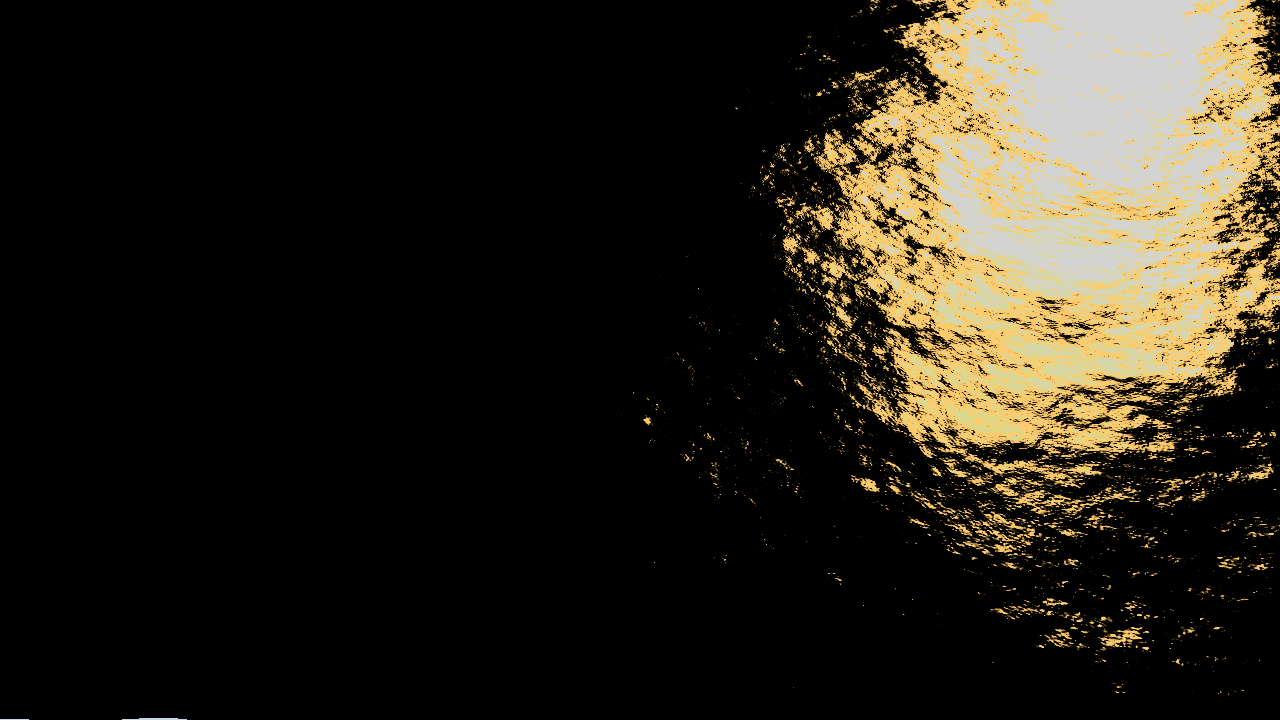
\includegraphics[width=0.48\textwidth]{figures/31-07-2017_10-47-08_ross.png}
	\label{fig:results:ross}
 }
 \hfill
 \subtop[Sky Contribution]
 {
  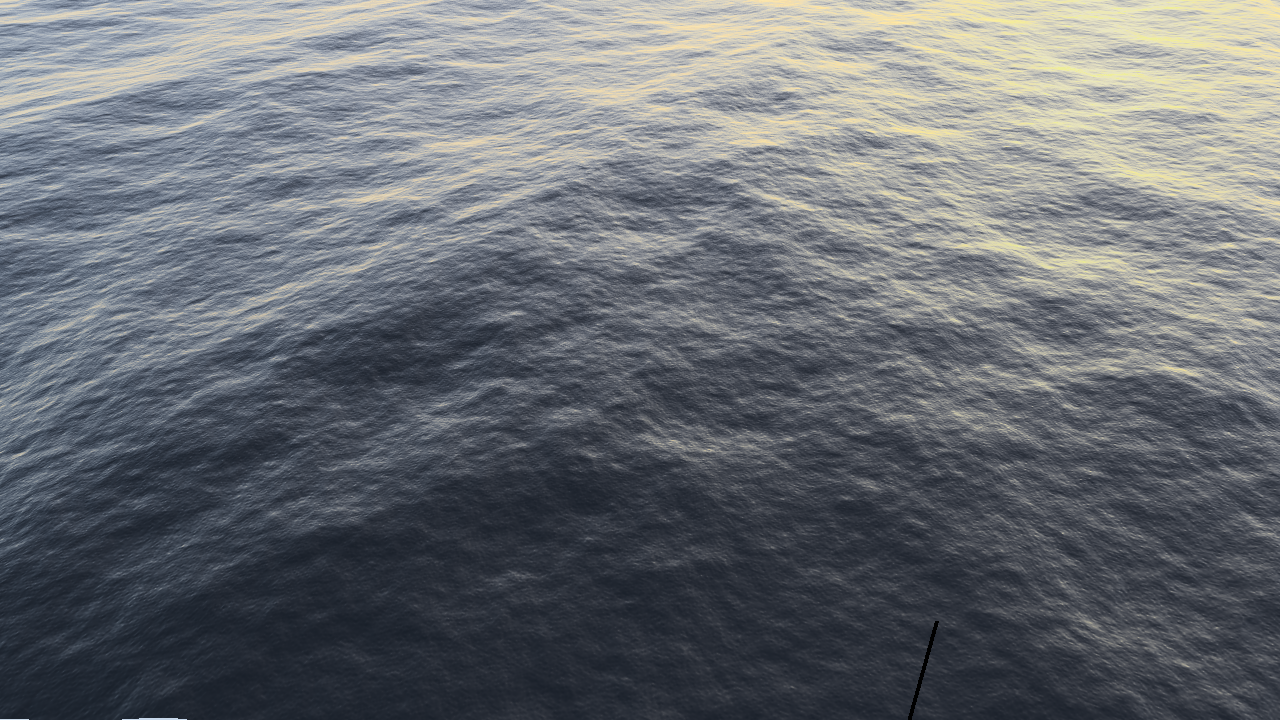
\includegraphics[width=0.48\textwidth]{figures/31-07-2017_10-47-08_sky.png}
	\label{fig:results:sky}
 }
 \hfill
 \subtop[Sea Contribution]
 {
  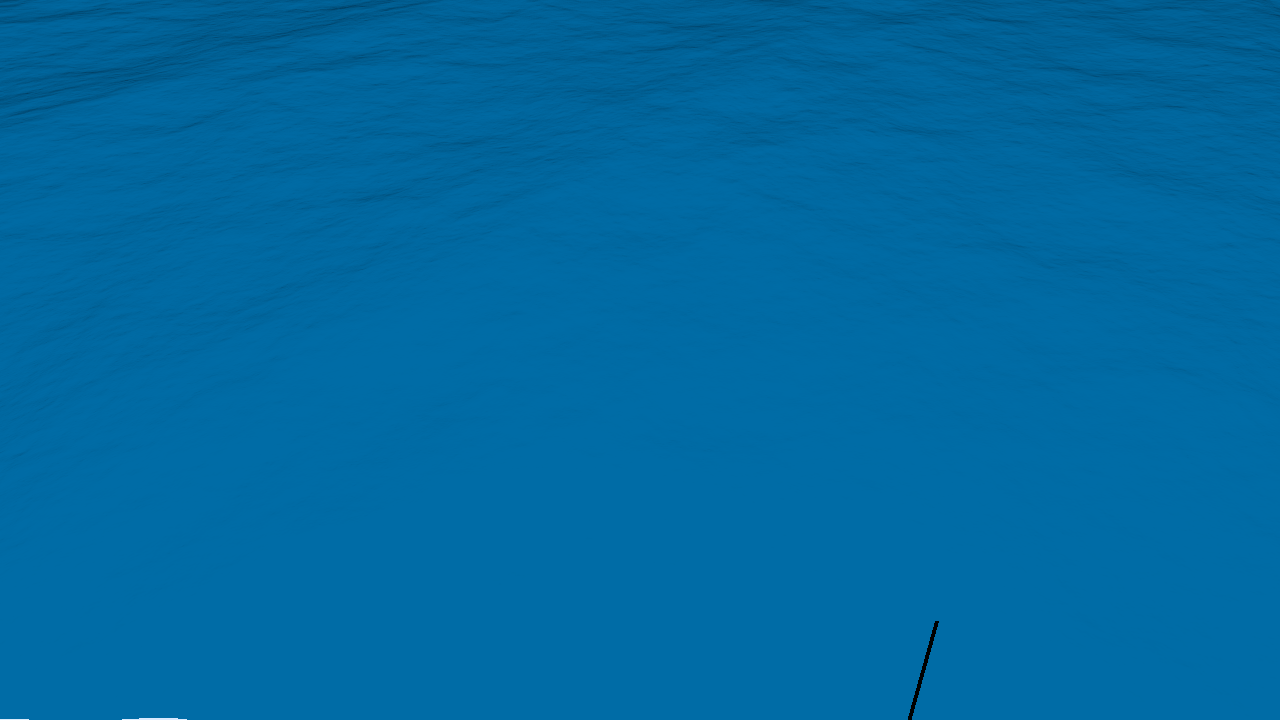
\includegraphics[width=0.48\textwidth]{figures/31-07-2017_10-47-08_sea.png}
	\label{fig:results:sea}
 }
 \hfill
 \subtop[Whitecaps Contribution]
 {
  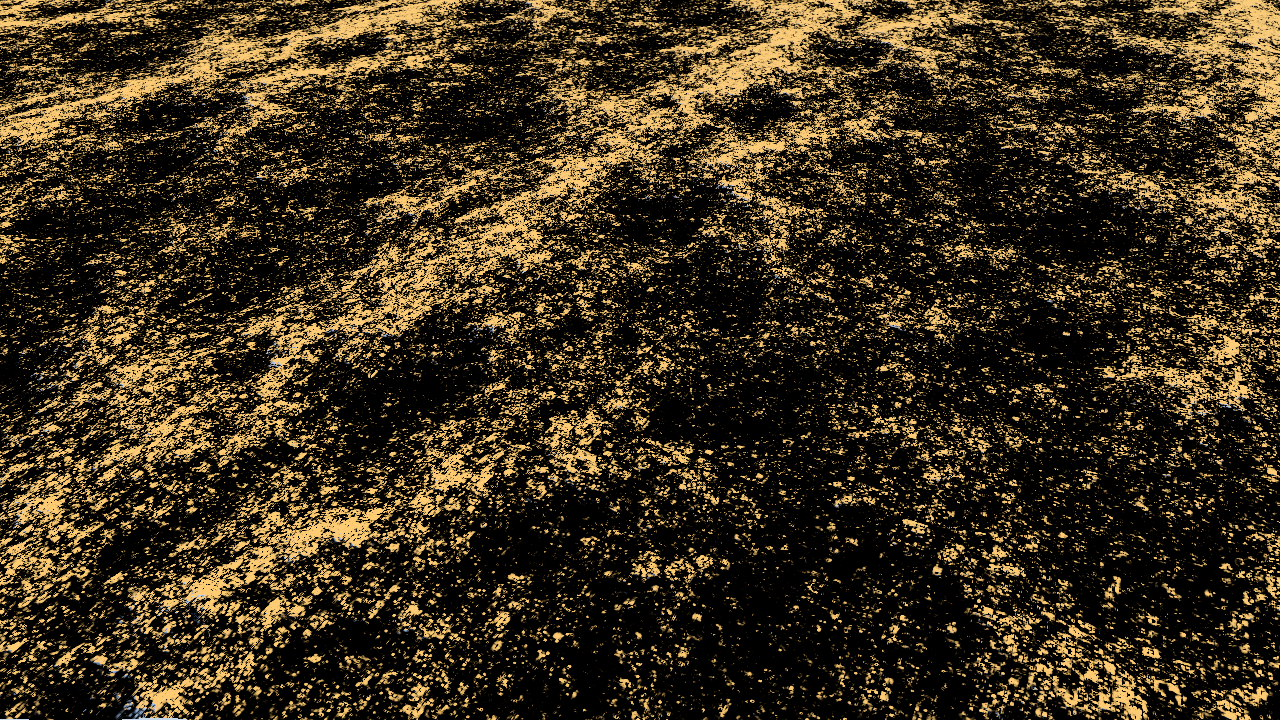
\includegraphics[width=0.48\textwidth]{figures/31-07-2017_10-47-08_whitecaps.png}
	\label{fig:results:whitecaps}
 }
 \hfill
 \subtop[Final Result]
 {
  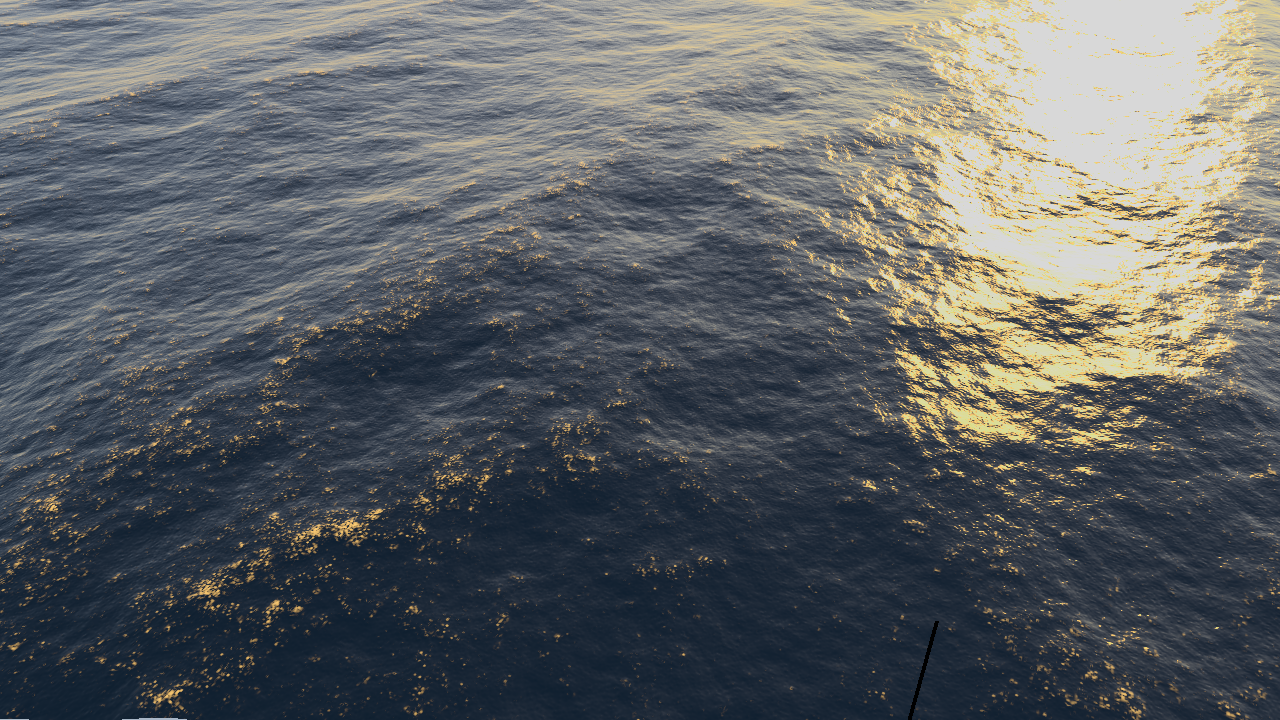
\includegraphics[width=\textwidth]{figures/31-07-2017_10-47-08_complete.png}
	\label{fig:results:complete}
 }
\caption{An overview of all ocean lighting terms involved in our implementation
of \citet{article:oceanlighting,misc:oceanlightingfft} and \citet{article:whitecaps}.
\subcaptionref{fig:results:ross} Sun light reflected by the water surface.
\subcaptionref{fig:results:sky} Sky light reflected by the water surface.
\subcaptionref{fig:results:sea} Light refracted from the water body.
\subcaptionref{fig:results:whitecaps} Whitecap foam.
\subcaptionref{fig:results:complete} All previous terms combined into the final
result.
}
\label{fig:results}
\end{figure}
%
Images of all partial terms involved in ocean lighting (specular by sun,
reflection of sky, refracted light, whitecaps)

Troubles with reflection vectors below horizon
Troubles with bright patches caused by reflection
Troubles with dark patches caused by reflection
Troubles with sundisk (XYZ to sRGB)

Tiling images

Comparison full resolution patterns vs multi-resolution scheme

Maybe different tonemapping settings